% (find-LATEX "2020-2-C2-intro.tex")
% (defun c () (interactive) (find-LATEXsh "lualatex -record 2020-2-C2-intro.tex" :end))
% (defun C () (interactive) (find-LATEXsh "lualatex 2020-2-C2-intro.tex" "Success!!!"))
% (defun D () (interactive) (find-pdf-page      "~/LATEX/2020-2-C2-intro.pdf"))
% (defun d () (interactive) (find-pdftools-page "~/LATEX/2020-2-C2-intro.pdf"))
% (defun e () (interactive) (find-LATEX "2020-2-C2-intro.tex"))
% (defun u () (interactive) (find-latex-upload-links "2020-2-C2-intro"))
% (defun v () (interactive) (find-2a '(e) '(d)))
% (defun cv () (interactive) (C) (ee-kill-this-buffer) (v) (g))
% (find-pdf-page   "~/LATEX/2020-2-C2-intro.pdf")
% (find-sh0 "cp -v  ~/LATEX/2020-2-C2-intro.pdf /tmp/")
% (find-sh0 "cp -v  ~/LATEX/2020-2-C2-intro.pdf /tmp/pen/")
%     (find-xournalpp "/tmp/2020-2-C2-intro.pdf")
%   file:///home/edrx/LATEX/2020-2-C2-intro.pdf
%               file:///tmp/2020-2-C2-intro.pdf
%           file:///tmp/pen/2020-2-C2-intro.pdf
% http://angg.twu.net/LATEX/2020-2-C2-intro.pdf
% (find-LATEX "2019.mk")
% (find-CN-aula-links "2020-2-C2-intro" "2" "c2m202intro" "c2m202i")
%
% Video:
% (find-ssr-links "c2intro" "2020.2-C2-intro")
% (code-video     "c2introvideo" "$S/http/angg.twu.net/eev-videos/2020.2-C2-intro.mp4")
% (find-c2introvideo "0:00")

% «.defs»			(to "defs")
% «.title»			(to "title")
% «.intro»			(to "intro")
% «.subst-zoomed»		(to "subst-zoomed")
% «.corrigir-igual»		(to "corrigir-igual")
% «.regra-da-cadeia»		(to "regra-da-cadeia")
% «.acrescentamos»		(to "acrescentamos")
% «.algumas-traducoes»		(to "algumas-traducoes")

\documentclass[oneside,12pt]{article}
\usepackage[colorlinks,citecolor=DarkRed,urlcolor=DarkRed]{hyperref} % (find-es "tex" "hyperref")
\usepackage{amsmath}
\usepackage{amsfonts}
\usepackage{amssymb}
\usepackage{pict2e}
\usepackage[x11names,svgnames]{xcolor} % (find-es "tex" "xcolor")
%\usepackage{colorweb}                 % (find-es "tex" "colorweb")
%\usepackage{tikz}
%
% (find-dn6 "preamble6.lua" "preamble0")
%\usepackage{proof}   % For derivation trees ("%:" lines)
%\input diagxy        % For 2D diagrams ("%D" lines)
%\xyoption{curve}     % For the ".curve=" feature in 2D diagrams
%
\usepackage{edrx15}               % (find-LATEX "edrx15.sty")
\input edrxaccents.tex            % (find-LATEX "edrxaccents.tex")
\input edrxchars.tex              % (find-LATEX "edrxchars.tex")
\input edrxheadfoot.tex           % (find-LATEX "edrxheadfoot.tex")
\input edrxgac2.tex               % (find-LATEX "edrxgac2.tex")
%
%\usepackage[backend=biber,
%   style=alphabetic]{biblatex}            % (find-es "tex" "biber")
%\addbibresource{catsem-slides.bib}        % (find-LATEX "catsem-slides.bib")
%
% (find-es "tex" "geometry")
\usepackage[a6paper, landscape,
            top=1.5cm, bottom=.25cm, left=1cm, right=1cm, includefoot
           ]{geometry}
%
\begin{document}

\catcode`\^^J=10
\directlua{dofile "dednat6load.lua"}  % (find-LATEX "dednat6load.lua")

% %L dofile "edrxtikz.lua"  -- (find-LATEX "edrxtikz.lua")
% %L dofile "edrxpict.lua"  -- (find-LATEX "edrxpict.lua")
% \pu

%  ____        __     
% |  _ \  ___ / _|___ 
% | | | |/ _ \ |_/ __|
% | |_| |  __/  _\__ \
% |____/ \___|_| |___/
%                     
% «defs»  (to ".defs")

% (find-LATEX "edrx15.sty" "colors-2019")
\long\def\ColorRed   #1{{\color{Red1}#1}}
\long\def\ColorViolet#1{{\color{MagentaVioletLight}#1}}
\long\def\ColorViolet#1{{\color{Violet!50!black}#1}}
\long\def\ColorGreen #1{{\color{SpringDarkHard}#1}}
\long\def\ColorGreen #1{{\color{SpringGreenDark}#1}}
\long\def\ColorGreen #1{{\color{SpringGreen4}#1}}
\long\def\ColorGray  #1{{\color{GrayLight}#1}}
\long\def\ColorGray  #1{{\color{black!30!white}#1}}
\long\def\ColorBrown #1{{\color{Brown}#1}}
\long\def\ColorBrown #1{{\color{brown}#1}}

\long\def\ColorShort #1{{\color{SpringGreen4}#1}}
\long\def\ColorLong  #1{{\color{Red1}#1}}

\def\frown{\ensuremath{{=}{(}}}
\def\True {\mathbf{V}}
\def\False{\mathbf{F}}

\def\drafturl{http://angg.twu.net/LATEX/2020-1-C2.pdf}
\def\drafturl{http://angg.twu.net/2020.2-C2.html}
\def\draftfooter{\tiny \href{\drafturl}{\jobname{}} \ColorBrown{\shorttoday{} \hours}}


%  _____ _ _   _                               
% |_   _(_) |_| | ___   _ __   __ _  __ _  ___ 
%   | | | | __| |/ _ \ | '_ \ / _` |/ _` |/ _ \
%   | | | | |_| |  __/ | |_) | (_| | (_| |  __/
%   |_| |_|\__|_|\___| | .__/ \__,_|\__, |\___|
%                      |_|          |___/      
%
% «title»  (to ".title")
% (c2m202introp 1 "title")
% (c2m202intro    "title")
%
% Aulas:
% 2021feb03 turma E1
% 2021feb04 turma C1

\thispagestyle{empty}

\begin{center}

\vspace*{1.2cm}

{\bf \Large Cálculo 2 - 2020.2}

\bsk

Aula 1: Introdução ao curso (e a EDOs e ao $[:=]$)

\bsk

Eduardo Ochs - RCN/PURO/UFF

\url{http://angg.twu.net/2020.2-C2.html}

\end{center}

\newpage


%  ___       _             
% |_ _|_ __ | |_ _ __ ___  
%  | || '_ \| __| '__/ _ \ 
%  | || | | | |_| | | (_) |
% |___|_| |_|\__|_|  \___/ 
%                          
% «intro»  (to ".intro")
% (c2m202introp 2 "intro")
% (c2m202intro     "intro")
\section{Introdução ao curso}

O curso de Cálculo 2 é principalmente sobre dois assuntos: {\bf
  integrais}, e {\bf equações diferenciais ordinárias}. Nós vamos
abreviar ``equação diferencial ordinária'' como ``EDO''; existem
também as {\sl equações diferenciais parciais}, ou EDPs, que são um
assunto beeem mais complicado.

\ColorRed{{\sl Integrais} são {\sl áreas}.} A expressão
$\Intx{a}{b}{f(x)}$ quer dizer ``a área sob a curva $y=f(x)$ entre
$x=a$ e $x=b$''. Mais visualmente,

% (find-latexinkscape-links "2020-1-C2/area-intro-1")

$$\Intx{a}{b}{f(x)} = \Area \left(
  \myvcenter{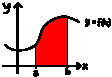
\includegraphics[width=4cm]{2020-1-C2/area-intro-1.pdf}}
  \right)
$$

\newpage

$$\Intx{a}{b}{f(x)} = \Area \left(
  \myvcenter{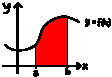
\includegraphics[width=4cm]{2020-1-C2/area-intro-1.pdf}}
  \right)
$$

Pra aprender a calcular essas áreas a gente vai ter que aprender a
aproximá-las por somas de retângulos -- um limite complicado! -- e os
detalhes vão dar um trabalhão... $\frown$

Repare, a área em vermelho é delimitada:

por cima pela \ColorRed{curva} $y=f(x)$,

pela esquerda pela reta $x=a$,

pela direita pela reta $x=b$,

por baixo pela reta $y=0$.

\newpage

{\bf Equações diferenciais} (lembre: ``ordinárias'' $→$ ``EDOs'') são
um pouco mais complicadas do que as equações que já sabemos
resolver...

\def\te{\text}

\msk

$\scalebox{0.90}{$
\begin{array}{rll}
 1) & x+2   = 5                   & \te{Equação de 1º grau} \\
 2) & x^2+3 = 7                   & \te{Eq.\ de 2º grau simples} \\
 3) & x^2+x = 6                   & \te{Eq.\ de 2º grau mais complicada} \\[5pt]
 4) & f'(x) = x^4                 & \te{EDO simples} \\
    & \text{ou: } \ddx f(x) = x^4 & \te{$f$ é a váriavel/incógnita!!!} \\
 5) & f'(x) = 2f(x)               & \te{EDO mais complicada} \\
 6) & f''(x) + f'(x) = 6f(x)      & \te{idem} \\
 7) & f'(x) = -1/f(x)             & \te{idem} \\
 8) & f'(x) = -x/f(x)             & \te{idem} \\
 \end{array}
 $}
$

\msk

Na passagem de (1) para (2) e (3) as equações ficaram mais complicadas
porque o $x$ passou a poder aparecer elevado ao quadrado.

No (4) estamos procurando uma \ColorRed{função} $f:\R→\R$ que obedeça
$f'(x) = x^4$ \ColorRed{para todo $x$}. Esse ``para todo $x$'' fica
\ColorRed{implícito}.

\newpage

\section{Chutar e testar}

Nosso primeiro método de resolver equações vai ser \ColorRed{chutar e
  testar} -- nós vamos chutar valores pra incógnita e ver se algum
deles é uma solução.

\begin{center}

\bf\Large

Aprender a \ColorRed{testar} vai ser
\underline{\underline{\underline{A}}} coisa

mais importante do curso.

\end{center}

Neste curso nós vamos usar duas coisas que não são padrão em cursos de
Cálculo 2:

1) Uma notação --- que normalmente só o pessoal de Computação aprende,
e só em cursos avançados... --- para \ColorRed{substituição de
  variáveis em expressões arbitrárias,}

2) Nós vamos usar a fórmula $e^{iθ} = \cosθ + i\senθ$ a beça.

\newpage

Nós vamos reescrever isto:

\msk

\begin{center}
\fbox{\begin{minipage}{7cm}
Se substituirmos $x$ por $10a+b$

e $y$ por $3c+4d$ em:
%
$$x^y + 2x$$
%
obtemos:
%
$$(10a+b)^{3c+4d} + 2(10a+b)$$
\end{minipage}}
\end{center}

\msk

deste jeito:

$$(x^y+2x) \bmat{x:=10a+b \\ y:=3c+4d} = (10a+b)^{3c+4d} + 2(10a+b)$$

\newpage

% «subst-zoomed»  (to ".subst-zoomed")
% (c2m202introp 7 "subst-zoomed")
% (c2m202intro    "subst-zoomed")

Repare: em
%
$$\scalebox{2.0}{$
  \begin{array}{l}
  (x^y+2x) \bmat{x:=10a+b \\ y:=3c+4d} \\[12pt]
  = (10a+b)^{3c+4d} + 2(10a+b)
  \end{array}
  $}
$$

a notação é
%
$$\text{(expressão original)[substituições] = (expressão nova)}$$

e cada uma das substituições é da forma:
%
$$\text{variável} := \text{expressão}$$


\newpage

A notação `$[:=]$' vai ser bem prática pra gente fazer hipóteses e
testá-las. Por exemplo, digamos que queremos testar se 2 e 3 são
soluções da equação $x+2=5$...
%
$$\begin{array}{rcl}
  (x+2=5)[x:=2] &=& (2+2=5) \\
                &=& (4=5) \\
                &=& \False \\[5pt]
  (x+2=5)[x:=3] &=& (3+2=5) \\
                &=& (5=5) \\
                &=& \True \\[5pt]
  \end{array}
$$

Note que os `$=$'s das expressões entre parênteses são
\ColorRed{comparações} -- como a operação `\texttt{==}' do \texttt{C}
-- e retornam ou $\True$ (``Verdadeiro'') ou $\False$ (``Falso'').

\newpage

% «corrigir-igual»  (to ".corrigir-igual")
% (c2m202introp 9 "corrigir-igual")
% (c2m202intro    "corrigir-igual")

{\bf ``Eu só vou corrigir os sinais de igual''}

Uma dos slogans que eu mais vou repetir quando estiver tirando dúvidas
ou corrigindo exercícios de vocês é ``\ColorRed{Eu só vou corrigir os
  sinais de igual}''.

Em Cálculo 1 muita gente se enrola com a fórmula da regra da cadeia --
porque se enrola na hora de substituir os `$f$'s, `$g$'s, `$f'$'s e
`$g'$'s nela... uma das fórmulas mais importantes, e mais difíceis de
acreditar, de Cálculo 2 é a da \ColorRed{Integração por Substituição},
que é BEEEEM pior do que a Regra da Cadeia. O \ColorRed{operador de
  substituição}, ``$[:=]$, que não tem nada a ver com a Integração por
Substituição, vai nos ajudar bastante a aplicar essas fórmulas passo a
passo sem a gente se perder.

Vamos precisar de alguns truques novos...

\newpage

% «regra-da-cadeia»  (to ".regra-da-cadeia")

{\bf Exemplo: regra da cadeia}

Primeiro vou inventar uma abreviação para a regra da cadeia.

\ColorRed{Obs: vários dos truques que vamos usar agora são inspirados
  em notações de Teoria da Computação e não são padrão!!! Não use eles
  em outros cursos!!! {\bf Os professores podem não entender e podem
    ficar putos!!!}}

\msk

O `$:=$' abaixo é uma \ColorRed{atribuição}, como o `\texttt{=}' do
\texttt{C}. A linha abaixo quer dizer: ``\ColorRed{a partir de agora}
o valor de $[RC]$ vai ser a \ColorRed{expressão} entre os parênteses
grandes.
%
$$[RC] \;\; := \;\; \left( \ddx f(g(x)) = f'(g(x))g'(x) \right)$$

\newpage

{\bf Exemplo: regra da cadeia (2)}

Continuando...
%
$$[RC] \;\; := \;\; \left( \ddx f(g(x)) = f'(g(x))g'(x) \right)$$

Então:
%
$$\begin{array}{rcl}
  [RC] \bmat{f := \sen} &=&
     \left( \ddx \sen(g(x)) = \sen'(g(x))g'(x) \right) \\[5pt]
  [RC] \bmat{f(u) := \sen u} &=&
     \left( \ddx \sen(g(x)) = \sen'(g(x))g'(x) \right) \\[5pt]
  [RC] \bmat{f(u) := u^4 \\ f'(u) := 4u^3 } &=&
     \left( \ddx (g(x))^4 = 4(g(x))^3g'(x) \right) \\
  \end{array}
$$

Repare que agora estamos substituindo o `$f$' \ColorRed{como se ele
  fosse uma variável} -- mas precisamos de gambiarras novas. No caso
do meio escrevemos $f(u) := \sen u$ ao invés de $f := \sen$, e...


\newpage

% «acrescentamos»  (to ".acrescentamos")
% (c2m202introp 12 "acrescentamos")
% (c2m202intro     "acrescentamos")

$$[RC] \;\; := \;\; \left( \ddx f(g(x)) = f'(g(x))g'(x) \right)$$

$$\begin{array}{rcl}
  [RC] \bmat{f := \sen} &=&
     \left( \ddx \sen(g(x)) = \sen'(g(x))g'(x) \right) \\[5pt]
  [RC] \bmat{f(u) := \sen u} &=&
     \left( \ddx \sen(g(x)) = \sen'(g(x))g'(x) \right) \\[5pt]
  [RC] \bmat{f(u) := u^4 \\ f'(u) := 4u^3 } &=&
     \left( \ddx (g(x))^4 = 4(g(x))^3g'(x) \right) \\
  \end{array}
$$
%
...e no caso de baixo acrescentamos uma linha ``$f'(u) := 4u^3$'' na
lista de substituições. Essa linha é uma \ColorRed{consequencia} da
linha ``$f(u) := u^4$'', e ela está lá só pra ajudar a gente a se
enrolar menos.

\newpage

{\bf Exercício}

Tente resolver as EDOs abaixo (de um dos primeiros slides) por chutar
e testar.

$$\begin{array}{rll}
 4) & f'(x) = x^4                 & \te{EDO simples} \\
    & \text{ou: } \ddx f(x) = x^4 & \te{$f$ é a váriavel/incógnita!!!} \\
 5) & f'(x) = 2f(x)               & \te{EDO mais complicada} \\
 6) & f''(x) + f'(x) = 6f(x)      & \te{idem} \\
 7) & f'(x) = -1/f(x)             & \te{idem} \\
 8) & f'(x) = -x/f(x)             & \te{idem} \\
 \end{array}
$$

Sugestão: comece testando $f(x) = x^3$, $f(x) = x^5$, $f(x) = 200x^5 +
42$, $f(x) = e^x$, $f(x) = e^{42x}$, $f(x) = e^{2x}$, $f(x)=e^{3x}$,
$f(x) = \sqrt{1-x^2}$, $f(x) = \sqrt{4-x^2}$.



\newpage

% «algumas-traducoes»  (to ".algumas-traducoes")
% (c2m202introp 14 "algumas-traducoes")
% (c2m202intro     "algumas-traducoes")

\thispagestyle{empty}

\begin{center}

\vspace*{2cm}

{\bf \Large Algumas traduções}

\end{center}

\newpage



%\printbibliography

\GenericWarning{Success:}{Success!!!}  % Used by `M-x cv'

\end{document}

%  __  __       _        
% |  \/  | __ _| | _____ 
% | |\/| |/ _` | |/ / _ \
% | |  | | (_| |   <  __/
% |_|  |_|\__,_|_|\_\___|
%                        
% <make>

 (eepitch-shell)
 (eepitch-kill)
 (eepitch-shell)
# (find-LATEXfile "2019planar-has-1.mk")
make -f 2019.mk STEM=2020-2-C2-intro veryclean
make -f 2019.mk STEM=2020-2-C2-intro pdf

% Local Variables:
% coding: utf-8-unix
% ee-tla: "c2m202intro"
% End:

